\documentclass[9pt,twocolumn,a4paper]{extarticle}

\usepackage[T1]{fontenc}
\usepackage[utf8]{inputenc}
\usepackage{mathptmx}
\usepackage{microtype}
\usepackage{geometry}
\usepackage{graphicx}
\usepackage{booktabs}
\usepackage{array}
\usepackage{natbib}
\usepackage{xcolor}
\usepackage{titlesec}
\usepackage[hidelinks]{hyperref}
\usepackage{xurl}
\usepackage{caption}
\usepackage{morefloats}
\usepackage{dblfloatfix}
\usepackage{amsmath}

\geometry{a4paper,top=25mm,bottom=25mm,left=20mm,right=20mm,columnsep=6mm}
\graphicspath{{figures/}}
\hypersetup{colorlinks=false,pdfborder={0 0 0}}
\captionsetup{font={stretch=1.0},labelsep=colon,justification=justified,singlelinecheck=true}

\titleformat{\section}{\normalfont\bfseries\filcenter}{\thesection.}{0.5em}{}
\titlespacing*{\section}{0pt}{\baselineskip}{\baselineskip}
\titleformat{name=\section,numberless}{\normalfont\bfseries\filcenter}{}{0pt}{}
\titlespacing*{name=\section,numberless}{0pt}{\baselineskip}{\baselineskip}
\titleformat{\subsection}{\normalfont\bfseries\raggedright}{\thesubsection}{0.5em}{}
\titlespacing*{\subsection}{0pt}{\baselineskip}{0.3\baselineskip}
\titleformat{\subsubsection}[runin]{\normalfont\bfseries}{\thesubsubsection}{0.5em}{}
\titlespacing*{\subsubsection}{0pt}{0.6\baselineskip}{0.5em}

\linespread{1.0}
\setlength{\parindent}{0pt}
\setlength{\parskip}{0.5\baselineskip}
\setlength{\textfloatsep}{\baselineskip}
\setlength{\floatsep}{\baselineskip}
\setlength{\intextsep}{\baselineskip}
\setcounter{dbltopnumber}{4}
\renewcommand{\dbltopfraction}{0.9}
\renewcommand{\dblfloatpagefraction}{0.7}
\renewcommand{\topfraction}{0.9}
\renewcommand{\bottomfraction}{0.9}
\renewcommand{\textfraction}{0.06}
\renewcommand{\floatpagefraction}{0.7}
\setlength{\bibhang}{0pt}
\setlength{\bibsep}{0pt}
\raggedbottom

% Generated by scripts/analysis/isprs_canonical_pipeline_v2.py
\newcommand{\ArchiveRecords}{33,378}
\newcommand{\RawArchiveRecords}{35,305}
\newcommand{\ExcludedArchiveRecords}{1,927}
\newcommand{\PrefectureAnchorRecords}{32,147}
\newcommand{\MunicipalityAnchorRecords}{1,231}
\newcommand{\MunicipalitySupportUnits}{452}
\newcommand{\CandidateToponymCount}{9,361}
\newcommand{\CandidateToponymPercent}{28.0}
\newcommand{\PlaceDescriptionCount}{25,023}
\newcommand{\PlaceDescriptionPercent}{75.0}
\newcommand{\HumanConditionCount}{16,066}
\newcommand{\HumanConditionPercent}{48.1}
\newcommand{\BroadInterfaceCount}{9,518}
\newcommand{\BroadInterfacePercent}{28.5}
\newcommand{\StrictInterfaceCount}{9,047}
\newcommand{\StrictInterfacePercent}{27.1}
\newcommand{\MedianAreaReduction}{97.5}
\newcommand{\MedianCoastSensitivity}{9.2}
\newcommand{\MedianWaterSensitivity}{0.1}
\newcommand{\PermutationCount}{10,000}
\newcommand{\RobustnessReplicates}{100}
\newcommand{\KappaWaterObservedPercent}{78.0}
\newcommand{\KappaWaterNullPercent}{23.1}
\newcommand{\KappaWaterOR}{15.72}
\newcommand{\KappaWaterQ}{0.0002}
\newcommand{\YureiDeathObservedPercent}{75.1}
\newcommand{\YureiDeathNullPercent}{16.1}
\newcommand{\YureiDeathOR}{23.01}
\newcommand{\YureiDeathQ}{0.0002}
\newcommand{\SnakeBoundaryOR}{1.49}
\newcommand{\SnakeBoundaryQ}{0.0002}
\newcommand{\KappaDistanceObserved}{0.371}
\newcommand{\KappaDistanceNull}{0.283}
\newcommand{\KappaDistanceOneSidedP}{0.9323}
\newcommand{\KappaDistanceTwoSidedP}{0.0892}


\begin{document}

\twocolumn[{%
\vspace*{0.5\baselineskip}
\begin{center}
{\fontsize{12}{14}\selectfont\bfseries
From Point Anchors to Geospatial Support: A Resolution-Aware Representation of Toponymic and Non-Toponymic Place Evidence in a Japanese Yokai Archive\par}
\vspace{1em}
{\fontsize{10}{12}\selectfont
Kosuke Shimizu\textsuperscript{1}, Hiroki Ichikura\textsuperscript{1}, Riri Ikebe\textsuperscript{2}, Mirai Hoshikawa\textsuperscript{1}\par}
\vspace{0.4em}
{\fontsize{9}{11}\selectfont
\textsuperscript{1} University of Tsukuba, 1-1-1 Tennodai, Tsukuba-shi, Ibaraki 305-8577, Japan -- shimizu@ai.iit.tsukuba.ac.jp\\
\textsuperscript{2} Japan Women's University, 2-8-1 Mejirodai, Bunkyo-ku, Tokyo 112-8681, Japan}
\end{center}
\vspace{1.2em}

{\noindent\textbf{Keywords:} Folklore geography, Geospatial support, Spatial humanities, Historical geocoding, Geographic resolution\par}
\vspace{\baselineskip}

{\noindent\textbf{Abstract}\par}
\vspace{0.4\baselineskip}
\noindent

Folklore archives often identify a broad administrative region while their summaries mix named places with non-toponymic descriptions of rivers, roads, dwellings, ritual sites, and boundaries. Treating an administrative representative point as an event location can therefore make the mapped evidence appear more precise than the source permits. We present a resolution-aware representation for \ArchiveRecords{} records from the Database of Folktales of Mysterious Phenomena and Yokai. It separates administrative support areas, candidate toponyms, non-toponymic place descriptions, geographic proximity, human-condition terms, derived interfaces, display anchors, and provenance. Rule-based coverage is \CandidateToponymPercent\% for candidate toponyms and \PlaceDescriptionPercent\% for place descriptions; these values are not extraction accuracy because no human gold labels are available. Rule-constrained local matching assigns municipality support to \MunicipalityAnchorRecords{} records across \MunicipalitySupportUnits{} units. Relative to prefecture support, municipality polygons reduce support area by a median \MedianAreaReduction\% and change sampled median coastline distance by \MedianCoastSensitivity{} km. Prefecture-stratified language associations recover expected Kappa--water and Yurei--death constructions, but these are construct checks rather than new folkloristic findings. A separate Kappa distance diagnostic does not support closer physical proximity to mapped major water. The contribution is an inspectable, failure-aware baseline that distinguishes display anchors from the support areas warranted by the archive.

\vspace{1.5em}
}]

\section{Introduction}

Japanese yokai traditions have long been widely acknowledged through local narratives, collected sources, and changing cultural classifications \citep{foster2024}. Digital archives make these materials searchable at scale, but a map adds claims that a catalogue does not: a point can suggest an event location, and a derived environmental label can suggest physical conditions. For short historical summaries, neither implication is safe unless the evidence supporting the geometry is retained.

The Database of Folktales of Mysterious Phenomena and Yokai, maintained by the International Research Center for Japanese Studies, provides bibliographic and regional metadata with short Japanese summaries \citep{nichibun2025}. A record may identify only a prefecture, mention one or more candidate toponyms, or describe a riverbank, route, dwelling, grave, shrine, livelihood, or boundary without naming a resolvable place. These signals differ in kind and resolution.

Historical geocoding compounds this problem because present administrative boundaries do not necessarily represent the places named in older sources. A representative point can be useful as a display anchor, but it is not evidence that the narrated event occurred there. We therefore treat resolution, support area, matching method, ambiguity, and provenance as explicit fields rather than as a calibrated probability.

This work represents vague folklore locations through separate evidence channels for administrative support areas, candidate toponyms, non-toponymic place descriptions, geographic context, human-condition terms, interface evidence, and support provenance. It shows how geographic summaries change when administrative support is refined, without treating representative coordinates as exact event locations. Three questions guide the study:

\textbf{RQ1 (Representation):} What evidence channels can be derived from vague folklore records while preserving the geographic support warranted by each record?

\textbf{RQ2 (Resolution sensitivity):} For records with uniquely matched municipality support, how do support area and coordinate-derived geographic features change relative to the prefecture-level baseline?

\textbf{RQ3 (Archive-language association):} Which category--place-function associations remain after controlling for prefectural composition?

The contributions are (i) an evidence-channel representation that separates textual and geographic support; (ii) an application to \ArchiveRecords{} archive records; (iii) a rule-constrained municipality-support subset; (iv) polygon-based resolution-sensitivity diagnostics; (v) prefecture-stratified archive-language association analyses with corrected inference and robustness checks; and (vi) an inspectable implementation whose reported numbers and figures are generated from one canonical result.

\section{Related Work}

\subsection{Folklore, Spatial Humanities, and Archive Bias}

Yokai categories are historically produced and transmitted rather than fixed biological taxa \citep{foster2024}. Spatial humanities likewise combines distant views with source criticism and close reading, while warning that mapped corpora inherit the coverage and classification decisions of their archives \citep{gregory2014}. Accordingly, record density in the present database is not interpreted as population prevalence or as a complete geography of Japanese folklore.

\subsection{Toponyms and Non-Toponymic Spatial Language}

Geoparsers generally detect toponyms and link them to gazetteer entries, as exemplified by HeidelPlace \citep{richter2017}. Japanese document-level work has developed richly annotated geographic-entity resources \citep{higashiyama2024}. However, locations can also be expressed through relations and common-noun descriptions that are not reducible to a named point \citep{stock2022}. Our representation retains both candidate toponyms and non-toponymic place descriptions; neither channel is treated as a validated extractor in the absence of a corpus-specific gold standard.

\subsection{Historical Geocoding and Region-Based Support}

Historical geocoding must accommodate temporal, textual, positional, and source uncertainty \citep{cura2018}. Gazetteer-linked annotation systems also preserve editorial intervention and source links \citep{simon2017}. The present study takes a more limited step: current administrative polygons provide support areas for records, and interior representative points provide display anchors. A matched current municipality is therefore a resolution refinement, not historical ground truth.

\subsection{Visualizing Evidential Limits}

Geospatial uncertainty research distinguishes sources of uncertainty and their visual encodings \citep{maceachren2005}. Digital-humanities visualizations can appear more objective than the underlying evidence and often omit uncertainty introduced during datafication \citep{panagiotidou2023}. Because the present pipeline has no calibrated probability, we describe it as ``resolution-aware'' and expose support basis, geometry, and ambiguity directly.

\section{Data}

The source is a local export acquired from the Nichibunken database by the repository's acquisition script. The canonical input contains \RawArchiveRecords{} raw records; cleaning retains \ArchiveRecords{} and excludes \ExcludedArchiveRecords{}: 141 summaries shorter than 10 characters and 1,786 records whose region is outside the Japanese prefecture set. A record is one database row, not a unique narrative event. Repeated narratives were not deduplicated because a defensible source-level equivalence rule is not available; their dependence is a limitation. Empty evidence channels are retained as missing rather than converted to negative evidence.

Prefecture strings are normalised to the repository's 47-name lookup. Categories follow the archive-derived field used by the existing acquisition pipeline. \textbf{TODO-AUTHOR:} document the acquisition date, full field mapping, category-construction rule, definition of the residual Other category, duplicate policy, source-period distribution, and treatment of malformed source metadata. The public database page reports 35,307 items as of April 2025 and notes that historical records can contain discriminatory language \citep{nichibun2025}; that count is not substituted for the local scrape count.

The source database's redistribution terms were not located in the supplied materials. Raw summaries and the locally generated qualitative-excerpt file must therefore remain non-public until the authors confirm permission. Current GADM boundaries are applied to potentially historical records only as contemporary support proxies. The analysis neither reconstructs historical boundaries nor dates individual geometries.

\section{Representation and Methods}

\begin{figure*}[t]
\centering
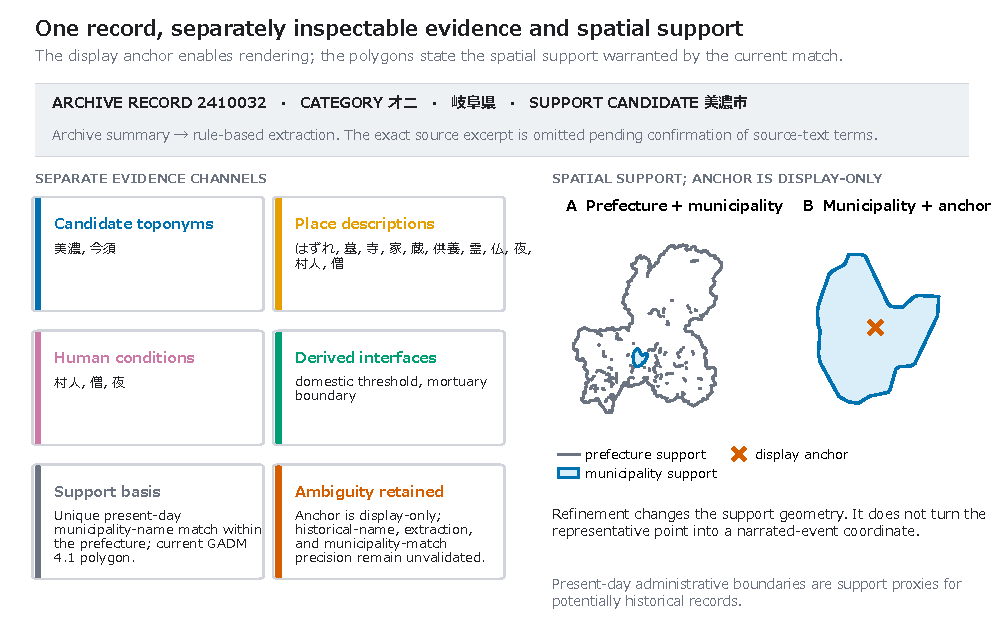
\includegraphics[width=\textwidth]{fig1_crown_jewel.pdf}
\caption{Crown-jewel view of one inspectable record. Original metadata and summary evidence are transformed into separate candidate-toponym, place-description, human-condition, interface, and provenance channels. The map distinguishes the prefecture support polygon, the rule-matched municipality support polygon, and the interior display anchor. The anchor is not asserted to be the narrated event location; the support basis and remaining ambiguity travel with the record.}
\label{fig:crown}
\end{figure*}

Figure~\ref{fig:crown} shows the distinction on which the pipeline is built. The Folklore Geospatial Support Model is a representation schema, not a predictive model. For record \(i\), it is
\[
S_i=(A_i,T_i,P_i,G_i,H_i,I_i,B_i),
\]
where \(A_i\) is administrative support, \(T_i\) candidate-toponym evidence, \(P_i\) non-toponymic place-description evidence, \(G_i\) coordinate-derived geographic context, \(H_i\) human-condition evidence, \(I_i\) derived interface evidence, and \(B_i\) the support basis and provenance. An anchor \(a_i\) is stored for display but is not part of the evidential support claim. Table~\ref{tab:model} specifies the source, rule, output resolution, ambiguity, provenance, and missing-data handling of each channel.

\begin{table*}[t]
\centering
\caption{Evidence-channel schema. Missing channels remain empty and do not erase evidence in other channels. ``Rule constrained'' describes matching restrictions, not measured precision.}
\label{tab:model}
\small
\setlength{\tabcolsep}{4pt}
\begin{tabular}{p{0.11\textwidth}p{0.15\textwidth}p{0.21\textwidth}p{0.16\textwidth}p{0.21\textwidth}}
\toprule
Channel & Source & Rule and output & Resolution & Ambiguity, provenance, and missing data \\
\midrule
\(A_i\) administrative support & Prefecture field; GADM 4.1 & Prefecture polygon; unique municipality polygon when matched & Prefecture or current municipality-like unit & Current-boundary source and matching method retained; prefecture fallback on no unique match \\
\(T_i\) candidate toponym & Japanese summary & GiNZA place-entity candidates; optional exact municipality candidate & Mention and candidate unit & All candidates retained; no calibrated confidence; empty if none detected \\
\(P_i\) place description & Summary and versioned dictionaries & Multi-label hydrology, mobility, boundary, livelihood, dwelling, death-ritual, taboo/time/weather terms & Textual, not geographic & Matched surface forms and dictionary hash retained; empty means no rule match \\
\(G_i\) geographic context & Support polygon, coastline, rivers, lakes & Continuous distances, densities, shares, and threshold proportions & Entire support polygon & Dataset, scale, projected coordinate reference system, and sampling seed retained \\
\(H_i\) human condition & Summary and dictionaries & Actor, action, or taboo/time/weather terms & Textual, not geographic & Matched terms retained; no inference about actual participants \\
\(I_i\) interface & Other evidence channels & Deterministic conjunctions such as hydrology with mobility & Record-level semantic metadata & Derivation path retained; not a physical site observation \\
\(B_i\) support basis & All stages & Method, source, resolution, candidate count, hashes & Record and run & Unknown values remain explicit; ``confidence'' is not reported \\
\bottomrule
\end{tabular}
\end{table*}

\subsection{Textual Evidence}

GiNZA 5.2.0 with spaCy 3.8.11 identifies candidate place entities in each summary \citep{matsuda2020,ginza520}. Versioned dictionaries independently identify place-function and human-condition surface forms. Place functions are hydrology, mobility, boundary, livelihood, dwelling, death ritual, and taboo/time/weather; textual landscape mentions separately record water, mountain, coast, boundary, and agrarian cues. These are multi-label textual features, not observed terrain.

Human-condition evidence is the union of actor, action, and taboo/time/weather terms. The broad human--environment interface is explicitly
\[
\begin{aligned}
E_i &= \mathrm{hydrology}\lor\mathrm{livelihood}\lor\mathrm{water}\\
    &\quad\lor\mathrm{mountain}\lor\mathrm{coast},\\
H_i &= \mathrm{actor}\lor\mathrm{action}\\
    &\quad\lor\mathrm{taboo/time/weather},\\
\mathrm{broad\ interface}_i &= E_i\land H_i .
\end{aligned}
\]
This definition makes every broad-interface record a subset of the human-condition records. Strict interfaces are named conjunctions: water crossing, waterside boundary, water-danger norm, mountain route, mountain boundary, coastal landing, domestic threshold, mortuary boundary, and water livelihood. The obsolete aggregate ``admin2 or boundary interface'' has no coherent set interpretation and is removed.

No human gold labels are available by design for this revision. We therefore report rule-based coverage, never precision, recall, \(F_1\), or validated extraction. Candidate toponym extraction, place-description extraction, human-condition extraction, interface derivation, and municipality matching are represented separately so that a future annotation study can evaluate them without changing the schema.

\subsection{Rule-Constrained Municipality Support}

GADM 4.1 level-2 units are filtered to municipality-like types Shi, Machi, Mura, SpecialWard, Capital, and Son \citep{gadm41}. The Japanese name field is \texttt{NL\_NAME\_2}; \texttt{NAME\_2} supplies English context. Names and summaries are whitespace-normalised. A direct summary match uses an official-name substring with a left-boundary constraint inside the record's prefecture. If that stage does not assign a unit, an exact candidate-toponym match is attempted. A record is refined only when the deduplicated candidate set contains one unit; multiple or same-named candidates remain at prefecture support. Direct summary matching has precedence, making the 329 direct matches and 902 entity-based matches mutually exclusive.

This procedure assigns municipality support to \MunicipalityAnchorRecords{} records across \MunicipalitySupportUnits{} unique units. Accepted record types are 929 Shi, 231 Machi, 53 Mura, and 18 SpecialWard; no accepted records use the other allowed types. Historical names are not resolved. GADM polygons are projected to EPSG:3095, and Shapely's interior representative point is transformed to WGS84 for display. The full polygon remains the evidential support.

\subsection{Polygon-Based Geographic Context}

Support metrics use GADM 4.1 polygons, Natural Earth 1:10m coastlines and lakes, and National Land Numerical Information W05 river centre-lines \citep{gadm41,naturalearth,mlitw05}. Distances and areas are computed in EPSG:3095. ``Major water'' is the union of the supplied lake boundaries and W05 river lines; river metrics use W05 lines only.

For support polygon \(P_i\) and feature geometry \(F\), the minimum distance is
\[
d_{\min}(P_i,F)=\min_{x\in P_i,y\in F}\|x-y\|.
\]
We additionally draw 128 deterministic area-uniform points \(x_{ij}\) per unique support and report the sampled median distance and the share meeting each threshold. Outputs include polygon area; minimum and sampled-median distance to coast, rivers, and major water; proportions within 0.5 km of major water, 2 km of a river, and 10 km of coastline; river and coastline density; and lake-area share. Sensitivity grids use coast thresholds 5, 10, and 20 km; river thresholds 1, 2, and 5 km; and water thresholds 0.25, 0.5, and 1 km. These thresholds are diagnostics rather than natural classes. No exclusive terrain classification or classification precedence is used.

\subsection{Archive-Language Associations}

RQ3 concerns semantic metadata within the archive, not physical geography. For each selected category--feature cell we report observed prevalence, the median null prevalence, observed-to-null ratio, prevalence difference, an odds ratio with a 95\% confidence interval, a two-sided empirical permutation value, and a Benjamini--Hochberg adjusted \(q\)-value \citep{benjamini1995}. The null shuffles category labels within prefectures \PermutationCount{} times, thereby preserving prefectural composition and category size. The empirical tail probability uses \((b+1)/(B+1)\). The screen contains 120 category--feature cells. Source-document blocking was not used because 50 joined records have missing or malformed source-group metadata; this remaining dependence limits inference.

Kappa--water and Yurei--death are prespecified construct checks: recovering known archive-language structures shows that the representation can encode them, not that the study discovered them. Snake/Dragon--strict boundary, Kappa--livelihood, and post-hoc mobility, dwelling, and taboo screens are exploratory. Surface-form leakage is reduced by masking category names, but semantic dependence is not claimed to be removed. Dictionary deletion is repeated \RobustnessReplicates{} times at each of 10\%, 20\%, and 30\%.

\section{Results}

\subsection{Evidence-Channel Coverage}

Figure~\ref{fig:coverage} and Table~\ref{tab:channels} report non-exclusive, rule-based coverage from the canonical result. Candidate toponyms occur in \CandidateToponymCount{} records (\CandidateToponymPercent\%), while non-toponymic place descriptions occur in \PlaceDescriptionCount{} (\PlaceDescriptionPercent\%). Human-condition evidence occurs in \HumanConditionCount{} (\HumanConditionPercent\%). The corrected broad interface contains \BroadInterfaceCount{} records (\BroadInterfacePercent\%) and is a verified subset of the human-condition set. The earlier count of 16,102 resulted from a broader and incompatible human-side definition; it is not retained.

\begin{figure}[t]
\centering
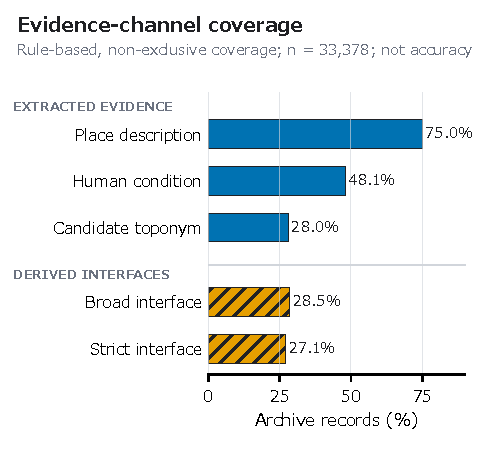
\includegraphics[width=\columnwidth]{fig2_evidence_coverage.pdf}
\caption{Rule-based coverage of non-exclusive evidence channels among \ArchiveRecords{} records. Bars report coverage, not extraction accuracy. The broad human--environment interface is defined as environmental evidence conjoined with actor, action, or taboo/time/weather evidence and is therefore a subset of the human-condition channel.}
\label{fig:coverage}
\end{figure}

\begin{table}[t]
\centering
\small
\begin{tabular}{lrr}
\toprule
Evidence channel & Records & Share \\
\midrule
Candidate toponym & 9,361 & 28.0\% \\
Non-toponymic place description & 25,023 & 75.0\% \\
Human condition & 16,066 & 48.1\% \\
Broad human--environment interface & 9,518 & 28.5\% \\
Strict derived interface & 9,047 & 27.1\% \\
\bottomrule
\end{tabular}
\caption{Coverage of separately represented evidence channels. Counts are rule-based coverage, not extraction accuracy; channels are non-exclusive. The denominator is \ArchiveRecords{} records.}
\label{tab:channels}
\end{table}


\subsection{Resolution Sensitivity of Polygon Support}

Figure~\ref{fig:resolution} and Table~\ref{tab:resolution} compare the \MunicipalitySupportUnits{} uniquely matched municipality polygons with their prefecture polygons. Municipality support reduces polygon area by a median \MedianAreaReduction\% (interquartile range 94.6--98.9\%). The median absolute change in sampled median coastline distance is \MedianCoastSensitivity{} km (4.2--17.0 km); for major water it is \MedianWaterSensitivity{} km (0.0--0.1 km after resolution-aware rounding). These are changes under administrative-support refinement, not corrected coordinates or errors against event locations.

\begin{figure}[t]
\centering
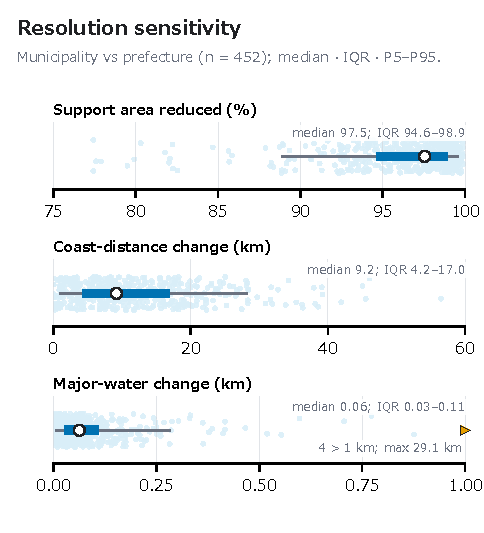
\includegraphics[width=\columnwidth]{fig3_resolution_sensitivity.pdf}
\caption{Resolution sensitivity for \MunicipalitySupportUnits{} municipality support polygons relative to their prefecture supports. The colour-vision-accessible panels show support-area reduction and absolute changes in sampled-median geographic-proximity metrics. Metrics use whole polygons and 128 deterministic area-uniform samples per support; no representative point is treated as ground truth.}
\label{fig:resolution}
\end{figure}

\begin{table}[t]
\centering
\small
\setlength{\tabcolsep}{3pt}
\begin{tabular}{p{0.52\columnwidth}rr}
\toprule
Metric & Median & IQR \\
\midrule
Support-area reduction (\%) & 97.5 & 94.6--98.9 \\
Coast-distance change (km) & 9.2 & 4.2--17.0 \\
Major-water-distance change (km) & 0.1 & 0.0--0.1 \\
\bottomrule
\end{tabular}
\caption{Resolution sensitivity for 452 uniquely matched municipality support polygons relative to their prefecture support polygons. Values are medians and interquartile ranges. Distances summarise 128 deterministic area-uniform sample points per support and are not errors against event-location ground truth.}
\label{tab:resolution}
\end{table}


\subsection{Archive-Language Associations}

Figure~\ref{fig:effects} and Table~\ref{tab:associations} replace the saturated standardised-residual heatmap with interpretable effect estimates. Kappa--water has 78.0\% observed versus 23.1\% median null prevalence (odds ratio 15.72, 95\% CI 13.82--17.89, \(q=0.0002\)); Yurei--death has 75.1\% versus 16.1\% (odds ratio 23.01, 20.47--25.87, \(q=0.0002\)). These strong values are construct checks for archive wording.

Among the exploratory cells, Snake/Dragon--strict boundary has an observed-to-null ratio of 1.34 and odds ratio \SnakeBoundaryOR{} (1.34--1.66, \(q=\SnakeBoundaryQ\)); Kappa--livelihood has a ratio of 1.47 and odds ratio 1.69 (1.50--1.91). Oni--mobility, Inugami--dwelling, and Hitodama--taboo/time/weather are post-hoc screens, not independent confirmation. Table~\ref{tab:examples} identifies the companion examples; \texttt{qualitative\_examples.csv} records the exact source excerpt, extracted terms, and derivation for one nontrivial record per reported exploratory feature. It remains local pending confirmation of source-text redistribution permission.

\begin{figure*}[t]
\centering
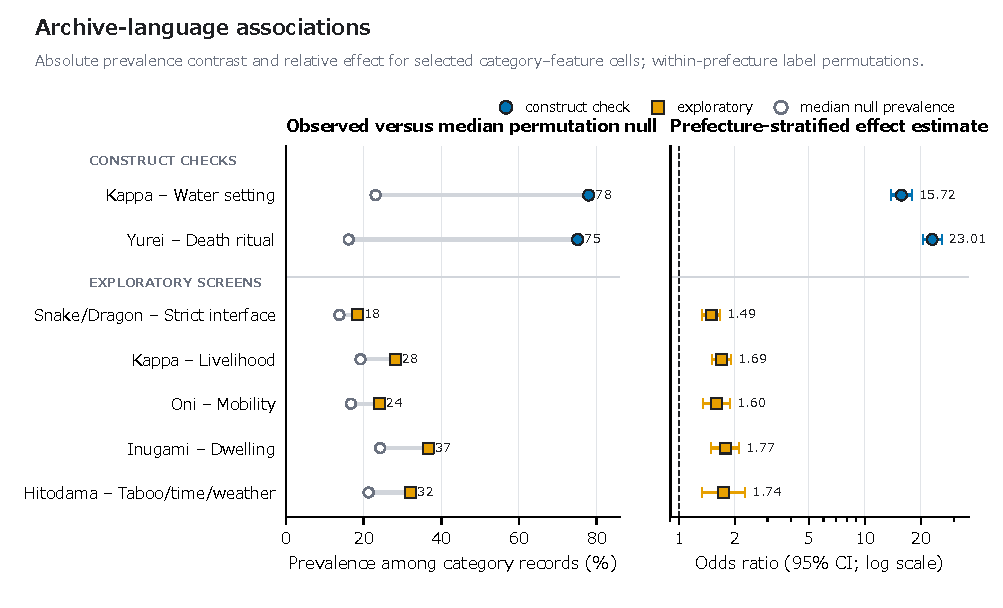
\includegraphics[width=0.88\textwidth]{fig4_archive_language_effects.pdf}
\caption{Prefecture-stratified archive-language effect estimates. Points are odds ratios and horizontal lines are 95\% confidence intervals; the reference line denotes no association. Kappa--water and Yurei--death are construct checks. Other rows are exploratory and describe archive-language co-occurrence, not physical ecological relationships.}
\label{fig:effects}
\end{figure*}

\begin{table*}[t]
\centering
\footnotesize
\setlength{\tabcolsep}{3pt}
\begin{tabular}{llrrrrrr}
\toprule
Category & Feature & Obs. \% & Null \% & O/E & OR & 95\% CI & $q$ \\
\midrule
Kappa & Water setting & 78.0 & 23.1 & 3.38 & 15.72 & [13.82, 17.89] & 0.0002 \\
Yurei & Death ritual & 75.1 & 16.1 & 4.65 & 23.01 & [20.47, 25.87] & 0.0002 \\
Snake/Dragon & Strict interface & 18.4 & 13.7 & 1.34 & 1.49 & [1.34, 1.66] & 0.0002 \\
Kappa & Livelihood & 28.2 & 19.2 & 1.47 & 1.69 & [1.50, 1.91] & 0.0002 \\
Oni & Mobility & 24.2 & 16.7 & 1.44 & 1.60 & [1.36, 1.88] & 0.0002 \\
Inugami & Dwelling & 36.6 & 24.3 & 1.50 & 1.77 & [1.49, 2.11] & 0.0002 \\
Hitodama & Taboo, time, or weather & 32.1 & 21.3 & 1.51 & 1.74 & [1.33, 2.28] & 0.0002 \\
\bottomrule
\end{tabular}
\caption{Prefecture-stratified archive-language associations. Null is the median prevalence under \PermutationCount{} within-prefecture label permutations. The $q$ value is Benjamini--Hochberg adjusted across 120 screened cells. Kappa--water and Yurei--death are construct checks; other rows are exploratory.}
\label{tab:associations}
\end{table*}


\begin{table}[t]
\centering
\caption{Traceability of qualitative examples. The exact Japanese summary excerpts and matched surface forms are stored in the local canonical file \texttt{qualitative\_examples.csv}; public redistribution is withheld pending author confirmation of source terms.}
\label{tab:examples}
\footnotesize
\setlength{\tabcolsep}{2pt}
\begin{tabular}{p{0.31\columnwidth}p{0.22\columnwidth}p{0.35\columnwidth}}
\toprule
Category--feature & Record ID & Derivation field \\
\midrule
Snake/Dragon--strict boundary & 1422080 & strict interfaces \\
Kappa--livelihood & C0410898-000 & livelihood + boundary cues \\
Oni--mobility & C0411171-000 & mobility + interface cues \\
Inugami--dwelling & 1231954 & dwelling + interface cues \\
Hitodama--taboo/time/weather & 1232238 & taboo/time + interface cues \\
\bottomrule
\end{tabular}
\end{table}

\subsection{Kappa Water-Distance Diagnostic}

The one-sided alternative is that Kappa-labelled municipality-supported records have a smaller median representative-point distance to mapped major water than expected after within-prefecture category shuffling. Among 1,231 municipality-supported records, 48 are Kappa. The observed median is \KappaDistanceObserved{} km, while the median of the \PermutationCount{}-permutation null distribution is \KappaDistanceNull{} km with a 95\% null interval of 0.218--0.377 km. The one-sided \(p\)-value for a smaller median is \KappaDistanceOneSidedP{} and the two-sided value is \KappaDistanceTwoSidedP{}; all \PermutationCount{} permutations are valid. Because the observed median exceeds the null median, the physical-proximity hypothesis is not supported. Repeated municipalities, rule-matched units, and use of representative points make this a limited negative diagnostic.

\subsection{Robustness Diagnostics}

Table~\ref{tab:robustness} shows that dictionary deletion gradually changes the full 120-cell ordering: median Spearman correlation is 0.975 at 10\% deletion, 0.940 at 20\%, and 0.895 at 30\%. Category-name masking removes 22,974 occurrences in 13,140 records and reduces surface-form leakage; it changes the Kappa--water observed-to-null ratio from 3.38 to 2.73 and Yurei--death from 4.65 to 3.57. It does not establish semantic independence. For the Snake/Dragon strict-boundary cell, the positive direction is retained in 100\%, 99\%, and 98\% of deletion replicates at the three rates; Kappa--livelihood retains it in 87\%, 85\%, and 70\%.

\begin{table}[t]
\centering
\caption{Dictionary-deletion robustness over \RobustnessReplicates{} deterministic replicates per rate. Spearman correlation compares the full category--feature effect-ratio ordering.}
\label{tab:robustness}
\small
\setlength{\tabcolsep}{3pt}
\begin{tabular}{rrrr}
\toprule
Deletion & Median $\rho$ & IQR & Min--max \\
\midrule
10\% & 0.975 & 0.942--0.987 & 0.878--0.999 \\
20\% & 0.940 & 0.916--0.963 & 0.846--0.994 \\
30\% & 0.895 & 0.852--0.925 & 0.665--0.979 \\
\bottomrule
\end{tabular}
\end{table}


\begin{table}[t]
\centering
\caption{Interface-definition ablation for the exploratory Snake/Dragon--boundary association. Construct-check rows are not repeated because these definitions do not alter their features.}
\label{tab:interface-ablation}
\small
\begin{tabular}{lr}
\toprule
Boundary-interface definition & O/E ratio \\
\midrule
Broad environmental \(\times\) boundary & 1.68 \\
Strict derived boundary interfaces & 1.34 \\
Hydrology/mountain boundary interfaces & 1.83 \\
\bottomrule
\end{tabular}
\end{table}

Table~\ref{tab:interface-ablation} demonstrates definition sensitivity rather than choosing a uniquely correct boundary construct. The full replicate distributions and effect-ratio summaries are retained in the canonical comma-separated value files.

\section{Discussion}

\textbf{RQ1.} The archive can be represented without collapsing all spatial evidence into one coordinate. Administrative polygons, candidate toponyms, non-toponymic place descriptions, geographic context, human-condition terms, derived interfaces, and provenance remain inspectable. The current implementation establishes representational coverage, not extraction accuracy.

\textbf{RQ2.} Municipality support produces much smaller evidential areas and materially different coastline summaries for the matched subset. The small median change in major-water distance reflects the density of the mapped river network and the sampled metric; it does not validate either administrative level as an event location. Polygon distributions are more faithful to the evidence than interpreting one display anchor, but present-day boundaries still remain proxies.

\textbf{RQ3.} Prefecture-stratified permutations recover known Kappa--water and Yurei--death archive-language associations and identify exploratory boundary, livelihood, mobility, dwelling, and taboo cells. The construct checks show that the schema captures obvious language structures; they are not new folklore findings. The exploratory cells require close reading and independent extraction validation before interpretation.

The distinction between textual and geographic evidence is decisive. A water term in a summary is textual landscape evidence; distance from a support polygon to a mapped river is geographic proximity. Conjoining them can produce a derived semantic interface, but it does not observe a local ecology. Likewise, dense archive coverage may reflect source collection, indexing, or repetition rather than regional folklore prevalence. Maps can over-objectify these choices, which is why the interface must show resolution, support polygon, display anchor, matching method, and source trace together.

Transfer to another archive requires a documented record unit, stable source identifiers, local-language place and function dictionaries, an appropriate historical or contemporary gazetteer, explicit redistribution terms, and a new human evaluation if extraction performance is to be claimed.

\section{Limitations}

No human gold standard is available, so precision, recall, \(F_1\), annotator agreement, and municipality-match precision are unknown. The rule dictionaries can miss obsolete names, shrine names, spelling variants, and implicit expressions, and can mistake common nouns or beings for places. Current administrative names cannot resolve many historical toponyms.

Records sharing a prefecture, municipality, source document, or repeated narrative are dependent. Prefecture-stratified permutations address only the first dependence; source-group blocking was not used because part of the local source metadata is malformed. The polygon sample is deterministic but finite, and W05 river vintages differ by region. Natural Earth 1:10m is appropriate for national context, not detailed local hydrology. No digital elevation model, slope, or terrain-position index is used.

The municipality subset is rule-matched rather than manually verified, and the representative-point distance diagnostic repeats shared municipal anchors. The analysis therefore does not establish exact event locations, coordinate accuracy, physical ecological relationships, diffusion from Kyoto, or population-level prevalence.

\section{Ethical Considerations}

This computational study involved no human participants. It uses historical source descriptions that may contain discriminatory language, as the database provider itself cautions \citep{nichibun2025}. Public displays should avoid unnecessary exposure of personal names, sacred sites, or small communities and should not turn uncertain narratives into precise-point claims or regional stereotypes.

GADM 4.1 permits academic and other non-commercial use but restricts redistribution and commercial use without permission \citep{gadm41}. Natural Earth data are public domain \citep{naturalearth}. The W05 river page identifies non-commercial conditions \citep{mlitw05}. \textbf{TODO-AUTHOR:} confirm and document the Nichibunken source-database terms, code licence, derived-data licence, exact W05 attribution required for redistribution, and whether any source excerpts may be published. No OpenStreetMap or Nominatim result is used by the canonical analysis; any future interface layer using OpenStreetMap must provide Open Database Licence attribution, and a public Nominatim service must not be used as a bulk reproducibility route.

Current boundaries are visibly labelled as present-day support proxies when applied to historical records. Archive density is not presented as folklore prevalence. \textbf{TODO-AUTHOR:} add the authors' required disclosure for any artificial-intelligence tools used in analysis or writing, following the destination venue's policy.

\section{Reproducibility}

The canonical command is:
\begin{quote}
\small\path{python scripts/analysis/isprs_canonical_pipeline_v2.py}
\end{quote}
It ran under Python 3.10.6 on Windows with GiNZA 5.2.0, ja-ginza 5.2.0, spaCy 3.8.11, GeoPandas 1.1.3, Shapely 2.1.2, pyproj 3.7.1, pandas 2.3.3, NumPy 1.26.4, Matplotlib 3.10.0, SciPy 1.13.0, and requests 2.32.5. The projected coordinate reference system is EPSG:3095. The base seed is 20260730; separate recorded seeds govern the association, distance, dictionary-deletion, and polygon-sampling stages. Runtime was 714.5 seconds on a 20-logical-core Windows host; \textbf{TODO-AUTHOR:} report memory and full hardware details.

The canonical directory contains \texttt{results.json}, versioned dictionary and configuration manifests, input and output SHA-256 hashes, record-level evidence fields, polygon metrics, threshold sensitivity, all permutation and robustness outputs, figure-generation scripts, generated LaTeX tables, and \texttt{number\_source\_map.csv}. The run records Git commit \texttt{76bb6b851bfbbd01f1c387123f9e2a1958bbd611} and an execution timestamp. The worktree was dirty, so this commit identifies the base repository rather than the complete revised state. Figure PDFs are vector outputs; PNG copies are previews.

\textbf{TODO-AUTHOR:} provide a public repository URL or archival DOI, commit the final revision, confirm Python and Node lock files, state code and derived-data licences, document a permitted source-data acquisition route, and report interface load time, latency, memory, browser, and Node version if interface performance is discussed. Non-redistributable source data should be acquired by the user and verified against the recorded hashes rather than bundled.

\section{Conclusion}

We represented \ArchiveRecords{} folklore records through separate administrative, toponymic, non-toponymic, geographic, human-condition, interface, and provenance channels. For RQ1, this schema preserves what kind of evidence supports each spatial interpretation, although its extractors remain unevaluated. For RQ2, municipality polygons substantially reduce support area and change polygon-derived coastline summaries relative to prefecture support; these changes measure resolution sensitivity, not accuracy. For RQ3, prefecture-stratified analysis recovers expected archive-language constructs and identifies exploratory cells for close reading, but it does not establish physical ecological relationships.

The next necessary step is a preregistered human evaluation of candidate toponyms, place descriptions, human-condition terms, interface derivations, and municipality matches, followed by source-aware models using verified historical place resolution. Until then, the defensible contribution is a failure-aware baseline that distinguishes display anchors from the support areas warranted by the available evidence.



\begingroup
\small
\raggedright
\bibliographystyle{plainnat}
\bibliography{refs_revised}
\endgroup

\end{document}
